\subsection{Descripción del problema.}

\vspace*{0.3cm}

En este problema, un cliente busca ofrecer un servicio particular sobre una
red existente de computadoras. Nuestra tarea consiste en elegir algunas de las
mismas, para utilizarlas como servidores formando un \textit{backbone} que
siga una tipología de red de tipo \textit{anillo}. Además, se requiere que
las demás computadoras de la red estén conectadas a algún servidor
perteneciente a este anillo, para poder tener acceso al mismo.

La red cuenta con conexiones entre algunos pares de equipos, pero
\textbf{por cada conexión utilizada se deberá pagar cierto costo
asociado al enlace utilizado}.

\medskip

El objetivo es elegir el anillo de servidores (indicando qué servidores y
enlaces lo representarán) y todas las demás conexiones necesarias, de
manera tal que las demás computadoras queden conectadas al anillo y el costo
asociado al uso de estos enlaces sea \textbf{mínimo}.

\vspace*{0.5cm}

\textbf{Ejemplo:}

En un sistema con 11 computadoras unidas con 13 enlaces distribuidas como
muestra la siguiente imagen:

\begin{figure}[htb]
  \begin{center}
      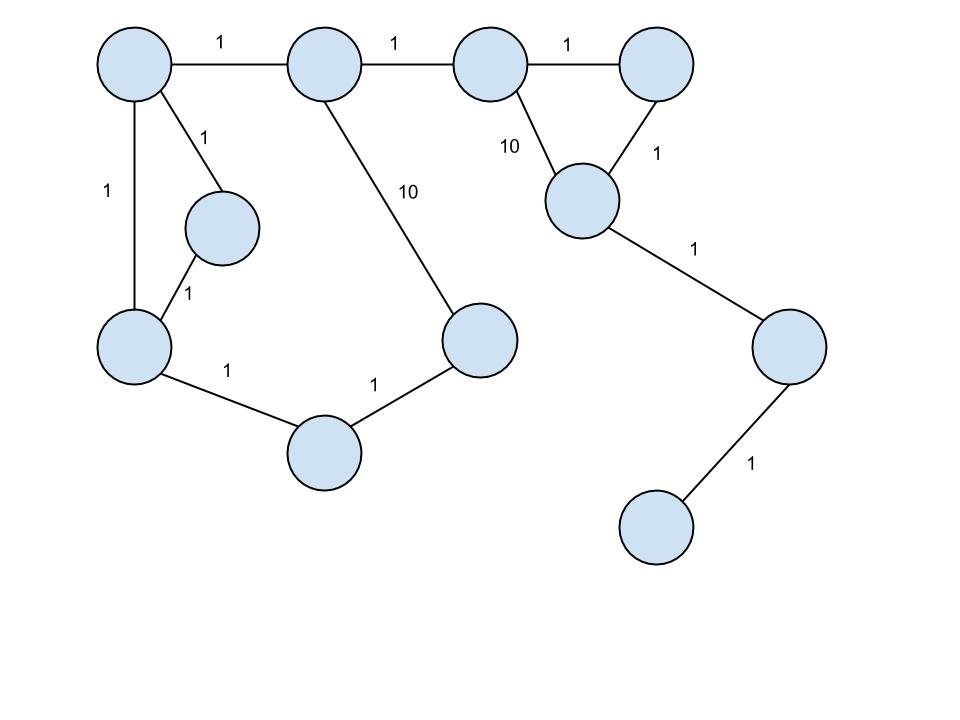
\includegraphics[scale=0.25]{imagenes/anillo-sin-hacer.jpg}
  \end{center}
  \caption{ejemplo de configuración de PC's y enlaces, con sus correspondientes costos.}
\end{figure}

\vspace*{0.5cm}

La solución óptima consiste en crear un anillo utilizando únicamente los
enlaces de costo 1 y dejar el resto de la red conectada de la siguiente
forma:

\begin{figure}[htb]
  \begin{center}
      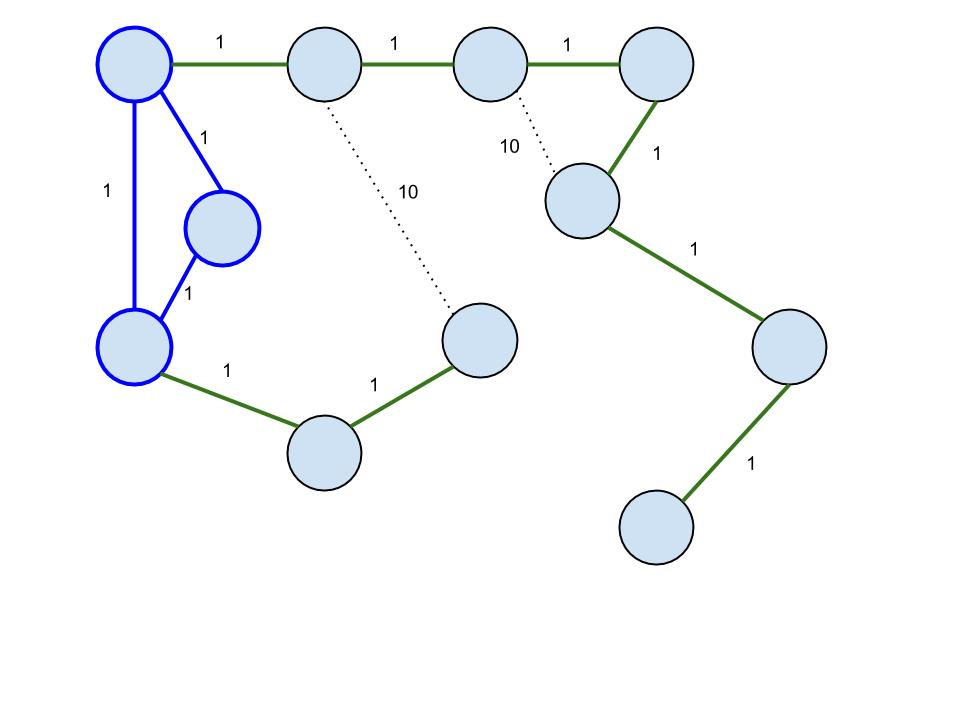
\includegraphics[scale=0.25]{imagenes/anillo-hecho.jpg}
  \end{center}
  \caption{ejemplo de anillo realizado.}
\end{figure}


\newpage
\subsection{Desarrollo de la idea y pseudocódigo.}

\vspace*{0.3cm}

En este problema, \textbf{trataremos a la red de computadoras como un grafo},
donde \textbf{las computadoras serán los vértices, las conexiones las aristas
y el peso de cada arista será el costo de hacer dicha conexión}.

Comenzaremos por corroborar que exista una solución. Para esto \textbf{el
grafo deberá ser conexo}, debe tener \textbf{al menos tantas aristas como
vértices} y \textbf{3 ó más vértices}. Si no fuese conexo, no se podrían
unir todas las computadoras. \textbf{Si tiene menos aristas que vértices},
el grafo sería un árbol, y con menos de 3 vértices \textbf{nunca podría formarse
un anillo}.

Suponiendo que tiene solución, se procederá a calcular el \textbf{árbol
generador mínimo} mediante el \textbf{algoritmo de Prim}. Para obtener el
anillo, \textbf{formaremos un ciclo agregando la arista de menor peso} no
incluída en el \textit{AGM}.


\begin{codebox}
\Procname{$\proc{tieneSolucion}(G)$}
\li \Return $(\proc{esConexo}(G)) \land
    \proc{\#}(\proc{aristas}(G)) \geq
    \proc{\#}(\proc{nodos}(G)) \land
    \proc{\#}(\proc{nodos}(G)) \geq 3$
\end{codebox}


\vspace*{0.3cm}


\begin{codebox}
\Procname{$\proc{esConexo}(G)$}
\li \Comment $\id{nodosPendientes}$ es una cola de nodos.
\li $\id{nodosPendientes} \gets \emptyset$
\li $\proc{agregarAtras}(nodosPendientes, primerNodo(G))$
\li \While $\id{nodosPendientes} \neq \emptyset$
\li     \Do
\li         $\id{nodo} \gets proc{pop}(nodosPendientes)$
\li         $\id{nodosVisitados[nodo]} \gets \const{true}$
            \For $\id{vecino} \in \proc{vecinos}(nodo)$
\li             \Do
                    $\proc{agregarAtras}(nodosPendientes, vecino)$
                \End
        \End
\li \Return $\proc{estanTodos}(nodosVisitados)$
\end{codebox}


\vspace*{0.3cm}


\begin{codebox}
\Procname{$\proc{prim}(G)$}
\li $\id{AGM} \gets \proc{nuevoGrafo}()$
\li $\proc{agregarNodo}(AGM, primerNodo(G))$

\li \While $\proc{cantidad}(nodos(AGM)) < \proc{cantidad}(nodos(G))$
      \Do
\li     $minima = \proc{min}(aristas con un nodo en AGM y el otro no)$
\li     $\proc{agregarAristaConSuNodo}(AGM, minima)$
      \End
\li \Return $\id{AGM}$
\end{codebox}


\vspace*{0.3cm}


\begin{codebox}
\Procname{$\proc{anillar}(G, peso : out)$}
\li $\id{AGM} \gets \proc{prim}(G)$
\li $\id{minima} \gets \proc{minimaNoIncluida}(AGM, G)$
\li $\id{peso} \gets \proc{peso}(AGM) + \proc{peso}(minima)$

\li $\id{enElAnillo} \gets \{minima\} \bigcup \proc{caminoMinimo}(nodo1(minima), nodo2(minima), AGM)$

\li $\id{fueraDelAnillo} \gets \proc{aristas}(AGM) \setminus \id{enElAnillo}$

\li \Return $< enElAnillo, fueraDelAnillo >$
\end{codebox}

\begin{codebox}
\Procname{$\proc{minimaNoIncluida}(AGM, G)$}
\li $\id{minima} \gets \proc{primerArista}(G)$
\li \For $\id{arista} \in \proc{aristas}(G)$
      \Do
\li     \If $\id{arista} \notin \proc{aristas}(AGM) \land
            \proc{peso}(arista) \leq \proc{peso}(minima)$
            \Do
\li            $\id{minima} \gets \id{arista}$
            \End
      \End
\li \Return $\id{minima}$
\end{codebox}


\newpage
\subsection{Justificación de la resolución y demostración de correctitud.}

\vspace*{0.3cm}

\textcolor{red}{\textbf{completar!}}

El problema requiere, dado una configuración de equipos en una red y sus
posibles conexiones con sus respectivos costos, armar una red con el menor
costo posible y la condición de que haya un anillo.

Este problema se reduce a, dado un grafo $G = (V, E)$ y $l: V \to
\mathbb{R}_{\geq 0}$ la función de peso de sus aristas, encontrar un
subgrafo $S = (V, E')$ con $E' \subseteq E$ de modo que la sumatoria del
peso sea mínima, el subgrafo sea conexo y tenga un solo circuito simple.

Primero que nada, notemos que el problema no siempre tiene solución si el
grafo no es conexo, pero también pueden no tener solución si es conexo: si
el grafo tiene el mínimo de aristas de modo que sea conexo (es decir, $m = n
- 1$), el grafo en cuestión es un árbol y por ende no tiene ciclos.
Excluidos estos casos, el problema tiene solución, pues es conexo y tiene al
menos un circuito simple (de no tenerlos, sería un árbol y ya vimos que esto
no puede suceder).

Conociendo el grafo es posible determinar si la instancia particular tiene
solución: solo basta ver que es conexo y tiene al menos tantas aristas como
vértices. Para determinar la conexión del grafo se lo recorre mediante
\textit{BFS} a partir de algún nodo. \textit{BFS} permite calcular los
caminos mínimos entre el nodo de inicio y todos los nodos en su misma
componente conexa. Luego, sabiendo la cantidad de nodos visitados al
finalizar \textit{BFS}, el grafo es conexo sí y solo sí la cantidad de nodos
visitados es igual a la cantidad de nodos del grafo. Si es conexo, como se
conoce la estructura del grafo, se sabe la cantidad de aristas y vértices de
este. Si $|E| \geq |V|$, se afirma que el problema tiene solución.

Partiendo ahora de la base de que la instancia tiene solución, veremos
que el algoritmo propuesto encuentra alguna de las posibles soluciones. En
efecto, si $A = (V_A, E_A)$ es el grafo solución de la instancia del
problema, se tiene que

\begin{itemize}
  \item $A$ es conexo.

  \item $A$ tiene un circuito simple.

  \item $\sum\limits_{e \in E_A} l(e)$ es mínima.
\end{itemize}

Consideremos $P = (V_P, E_P)$ el árbol generador mínimo obtenido al aplicar
el algoritmo de Prim a $G$ y sea $m \in E \setminus E_P$ tal que $l(m) \leq
l(e) \; \forall e \in E \setminus E_P$. Llamemos $S = (V_S, E_S)$, con $V_S
= V_P$ y $E_S = E_P \cup \{m\}$, es decir, $S$ es el grafo obtenido al
agregar la arista $m$ a $P$. $S$ es subgrafo de $G$ pues $P$ lo era y $w \in
E \setminus E_P$, y por ende $V_S = V_P = V$ y $E_S \subseteq E$. Veamos
ahora que $S$ es en efecto una solución al problema:

\begin{itemize}
  \item $S$ es conexo: $P$ es conexo y $E_S = E_P$, $S$ es el resultado de
  agregarle una arista a $P$, por lo tanto, para cualquier par de vértices
  $v, w \in V_S$, si $C$ es el camino en $P$ entre $v$ y $w$, $C \in E_S$
  pues $C \in E_P$.
  \item $S$ tiene un circuito simple: como $P$ es un árbol, por definición,
  como $w \in E \setminus E_P$, al agregar $m$ a $E_P$ se obtiene un
  circuito simple.
  \item $\sum\limits_{e \in E_S} l(e)$ es mínima: supongo que no, es decir,
  dado $A = (V_A, E_A)$ un grafo solución de la instancia del problema,
  $\sum\limits_{e \in E_S} l(e) > \sum\limits_{e \in E_A} l(e)$.
\end{itemize}


\newpage
\subsection{Análisis de complejidad.}

\vspace*{0.3cm}

Para el análisis de complejidad nos basaremos en el pseudocódigo de la función
\textsc{sePuedeAnillar}, correspondiente al ítem \textbf{5.2}.

vector
list
queue
tuple

\begin{enumerate}
  \item La operación \verb|size|, realizada sobre el contenedor \verb|vector| de la
  \textit{STL}, toma tiempo constante $O(1)$. Por lo tanto, cada vez que sea utilizada
  como parte de la implementación de algún algoritmo, asumiremos que no agrega complejidad
  adicional a la ya existente.

  \item La operación \verb|resize|, realizada sobre el contenedor \verb|vector| de la
  \textit{STL}, toma tiempo lineal $O(n)$. Por lo tanto, cada vez que sea utilizada
  como parte de la implementación de algún algoritmo, agregaremos (ó multiplicaremos por)
  $n$ a la complejidad ya existente.

  \item En la línea 1, la complejidad de \textsc{tieneSolucion} depende sólamente de
  la complejidad de \textsc{esConexo} (que evaluaremos a continuación), ya que
  \textsc{\#(aristas)} y \textsc{\#(nodos)} se calculan en tiempo constante $O(1)$
  (son datos que se cargan con los valores de entrada, $n$ y $m$) y compararlos es
  también $O(1)$ (estamos comparando enteros de tamaño acotado).
  Por lo tanto, el costo de preguntar si $G$ tiene ó no solución es $O(n^2)$.

  Retornar un valor booleano ($true, false$) toma tiempo constante, $O(1)$. Por lo tanto,
  la complejidad total de \textsc{sePuedeAnillar} surge de la suma entre la complejidad de
  \textsc{tieneSolucion} (vimos que es $O(n^2)$) y la complejidad de \textsc{completarAnillo}.

  \item La complejidad de \textsc{tieneSolucion}, como dijimos anteriormente, depende
  únicamente del costo de la función \textsc{esConexo}, ya que el resto de la conjunción
  toma tiempo constante y no agrega complejidad extra. Por lo tanto, estudiaremos la
  complejidad de \textsc{esConexo}. Esta función itera sobre los vértices de $G$.
  Dado un vértice, podemos saber cuáles son las aristas que inciden sobre el (es decir,
  quiénes son sus vértices vecinos). En nuestra implementación utilizamos una \textit{matriz de
  pesos} de tamaño $n^2$ (se trata de un vector con una posición por cada nodo, donde a su vez,
  tenemos otro vector por cada posición). De esta manera, en la posición $i,j$ de la matriz,
  tenemos un entero que representa el peso de la conexión entre el nodo $i$ y el nodo $j$ (y viceversa).
  En el caso donde no haya un peso definido (por no encontrarse entre los datos de entrada) el valor
 de dicha posición es $-1$ (en el pseudocódigo, este valor se representa como $\infty$).
  Por lo tanto, iterar sobre todas las aristas de $G$ toma tiempo
  cuadrático, $O(n^2)$ (debemos iterar siempre sobre la matriz entera).
\end{enumerate}

A medida que vamos encontrando valores de pesos de conexiones válidos, marcamos la posición
correspondiente al nodo visitado en el vector de nodos de $G$.

uego de terminar de iterar sobre la matriz, chequeamos si efectivamente todos los nodos de $G$
fueron visitados, lo cual implica que para cualquier par de nodos de $G$ hay camino y por lo
tanto, es conexo. Esto es lineal en la cantidad de nodos de $G$, $O(n)$.

Luego, la complejidad de \textsc{esConexo} es $O(n^2) + O(n) = O(n^2)$.

\newpage
\subsection{Experimentación y gráficos.}

\vspace*{0.3cm}

\subsubsection{Test 1 - benchmark caso aleatorio}

\textcolor{red}{\textbf{completar!}}


\newpage
\subsubsection{Test 2 - benchmark del peor caso}

\textcolor{red}{\textbf{completar!}}


\newpage
\subsubsection{Test 3 - benchmark del mejor caso}

\textcolor{red}{\textbf{completar!}}
